\chapter{LCD Timings}%
\label{cha:lcd_timings}

Because timings for the LCD are important, this chapter shows the measured
timings after the display starts running. They (mostly) corresponds to~\cite[LCD
data sheet]{ortustechlcd}. The timings needs to be configured within
the \gls{DTS} and are in this way the input for the video \gls{DRM} driver.

\textbf{NOTE:}\@ The DRM driver is patched by the Telair International GmbH to
be complaint to some silicon erratas belongs to the MCUs DRM peripheral
(see~\cite{TI_am335x_errata} and \fullref{cha:patches}). Otherwise the LCD
type used in this project would no work. V-Sync is an \textit{active low}
dataline.

\newpage
\section{H-Sync timings}%
\label{sub:sync_timings}

The following graphics show the timings by an logic analyzer on the horizontal
signal dataline (H-Sync) after the LCD gets running.
\begin{figure}[h!]
\begin{center}
    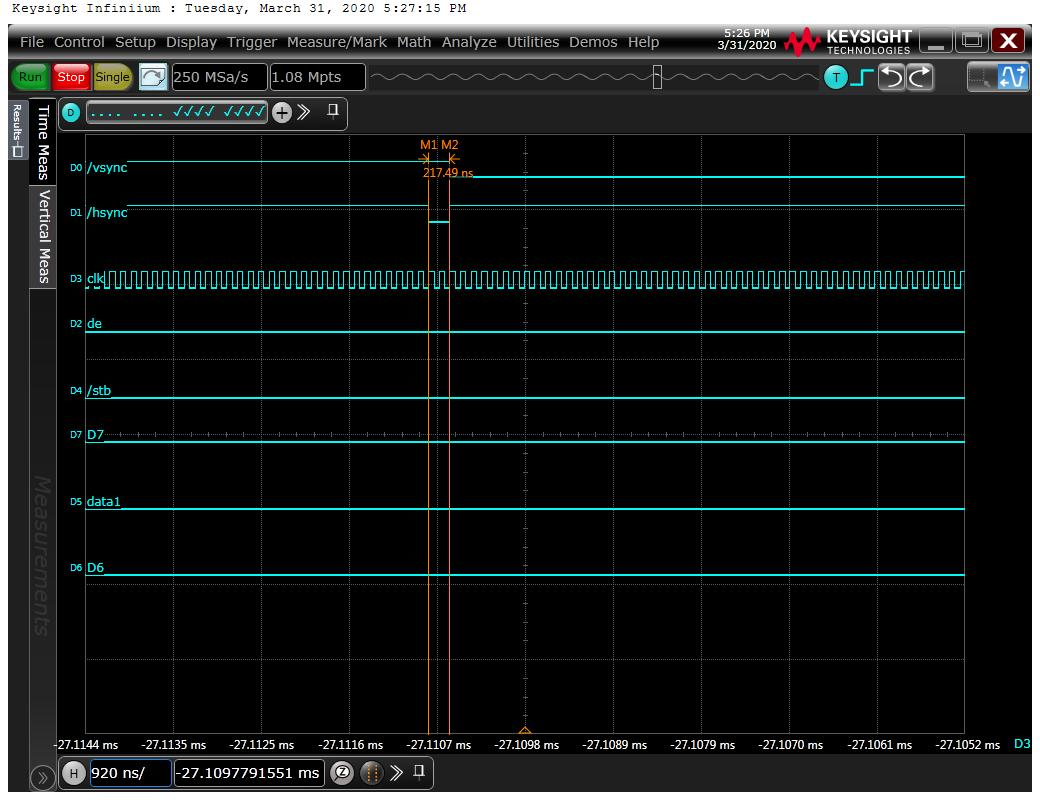
\includegraphics[width=14cm]{pictures/lcd_timings/hsync_length.jpg}
\end{center}
\caption{Length time of one low active H-Sync phase}
\label{fig:hsync_active_time}
\end{figure}

\newpage

\begin{figure}[ht]
\begin{center}
    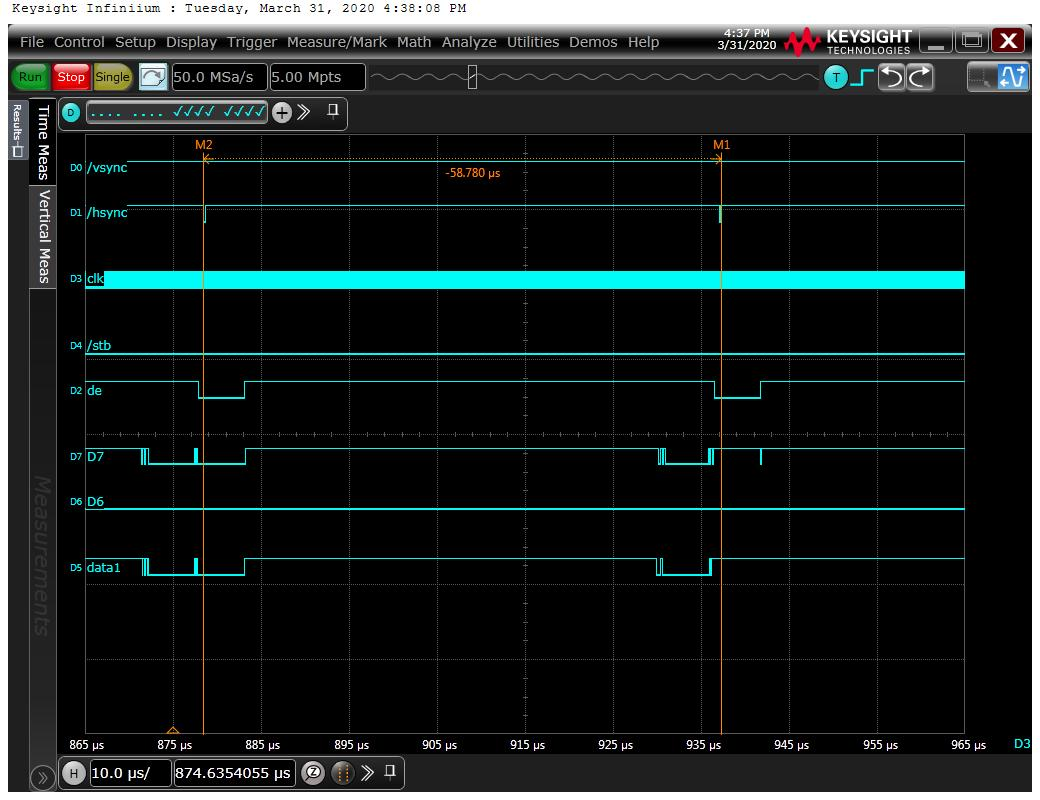
\includegraphics[width=14cm]{pictures/lcd_timings/hsync_periode.jpg}
\end{center}
\caption{Time length of one howl ht-Sync period}
\label{fig:hsync_period}
\end{figure}

\newpage
\section{V-Sync timings}%
The following graphics show the timings by an logic analyzer on the horizontal
signal dataline (V-Sync) after the LCD gets running. V-Sync is an \textit{active
low} dataline.
\label{sub:vsync_timings}
\begin{figure}[!h]
\begin{center}
    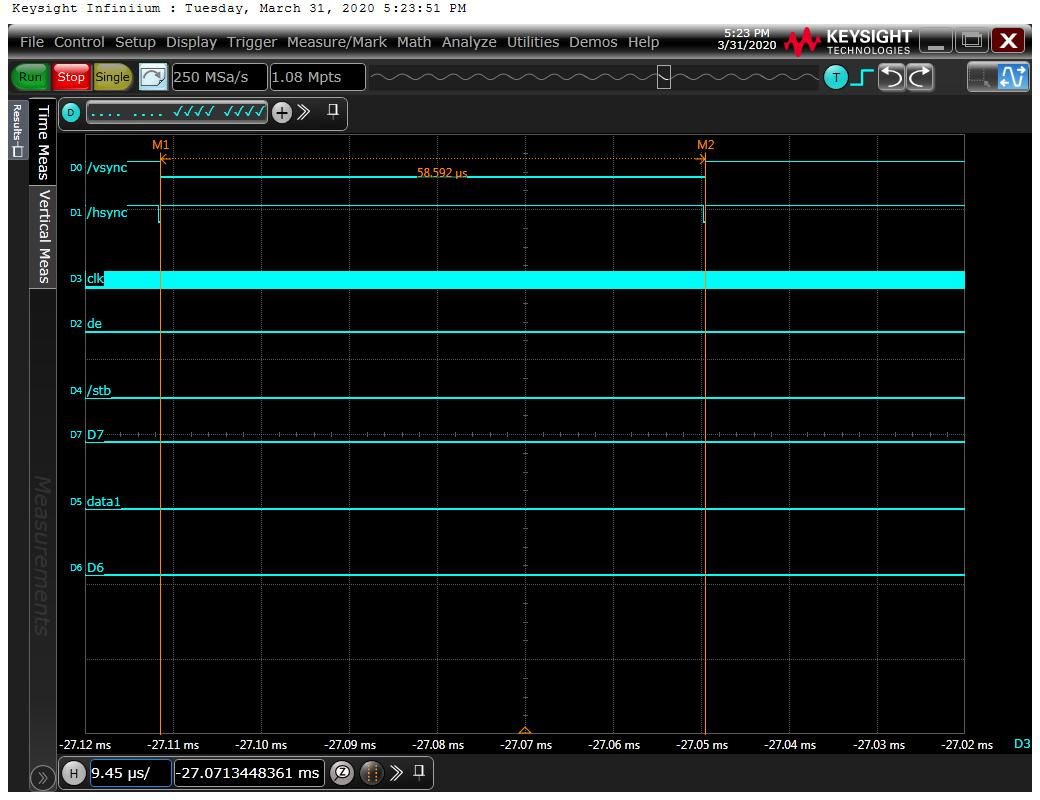
\includegraphics[width=14cm]{pictures/lcd_timings/vsync_length.jpg}
\end{center}
\caption{Length time of one low active V-Sync phase}
\label{fig:vsync_active_time}
\end{figure}
\newpage
\begin{figure}[ht]
\begin{center}
    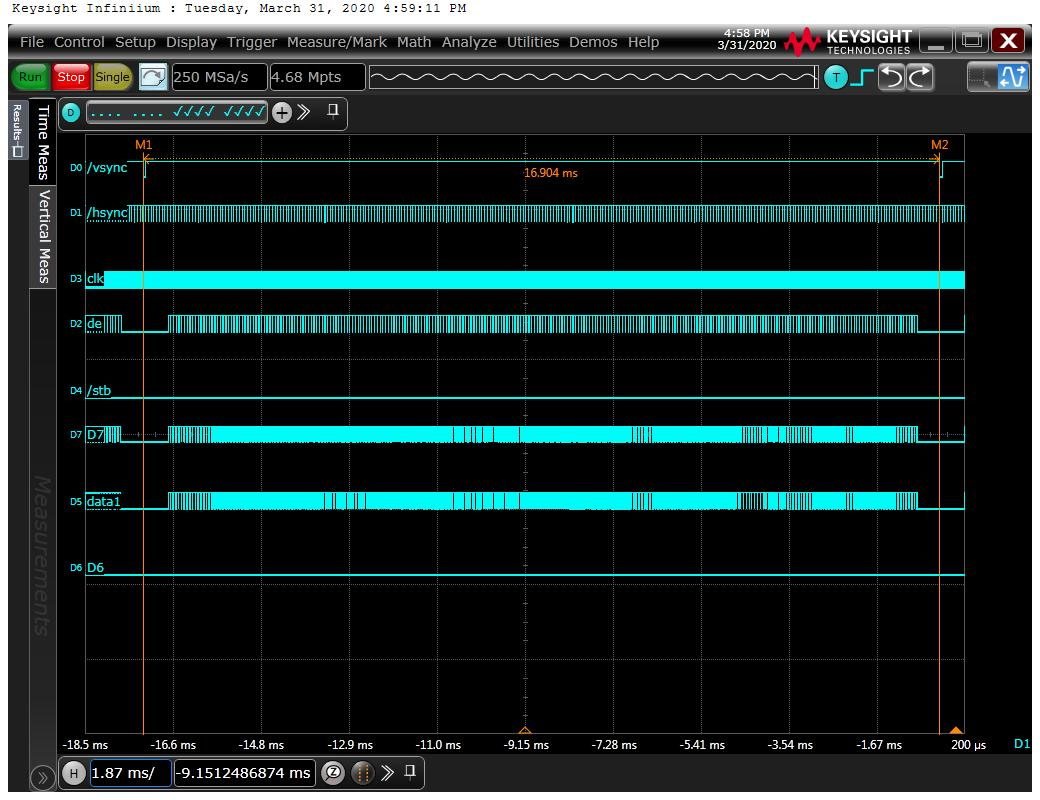
\includegraphics[width=14cm]{pictures/lcd_timings/vsync_periode.jpg}
\end{center}
\caption{Time length of one howl V-Sync period}
\label{fig:one_vsync_period}
\end{figure}

\pagebreak
\section{One Clock time length}%
The following graphics show the timings by an logic analyzer on the clock
after the LCD gets running. Because of falling and rising edge triggering der
timing of clock signal is important.
\label{sub:clock_time_length}
\begin{figure}[h!]
\begin{center}
    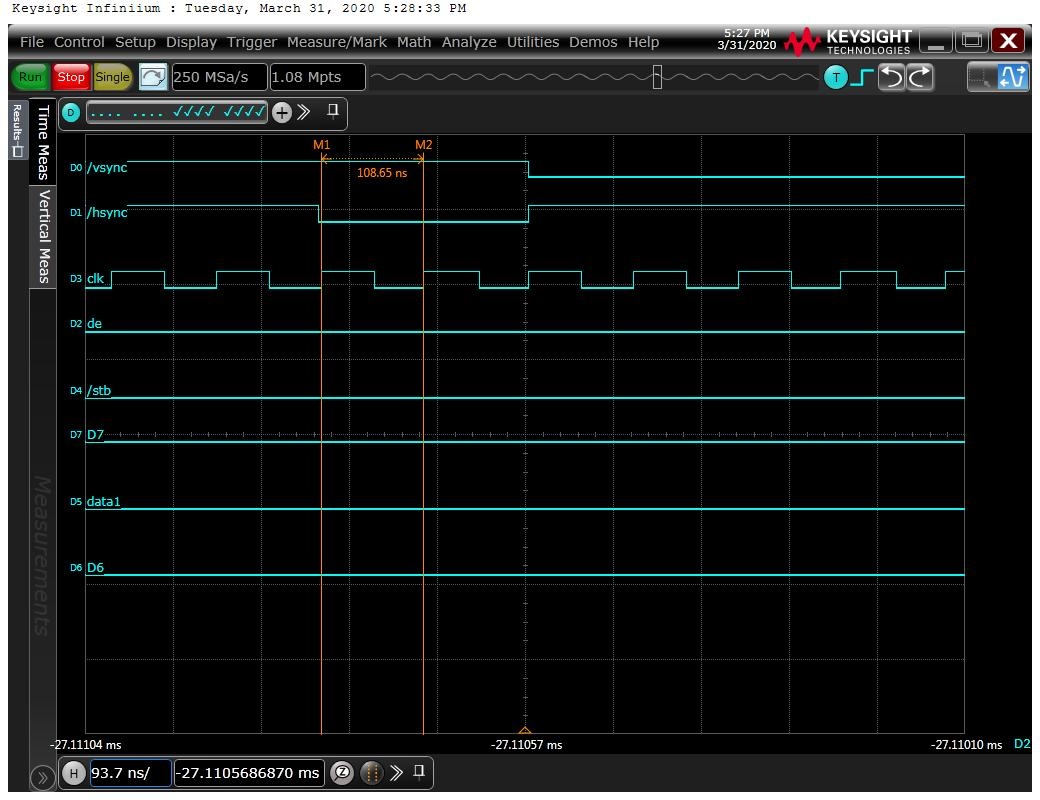
\includegraphics[width=14cm]{pictures/lcd_timings/periode_time_1clk.jpg}
\end{center}
\caption{Time length of one clock period}
\label{fig:one_clock_time}
\end{figure}


\pagebreak
\section{H-Sync vs. DE signal}%
\label{sub:other_measured_lcd_timings}
The following graphics show the timings by an logic analyzer on the H-Sync
signal dataline and the data Enable Data line (DE) to get the system
running. Note: The H-Sync is active low and the DE active high both according to
the datasheet and needs to be in time.

\begin{figure}[h!]
\begin{center}
    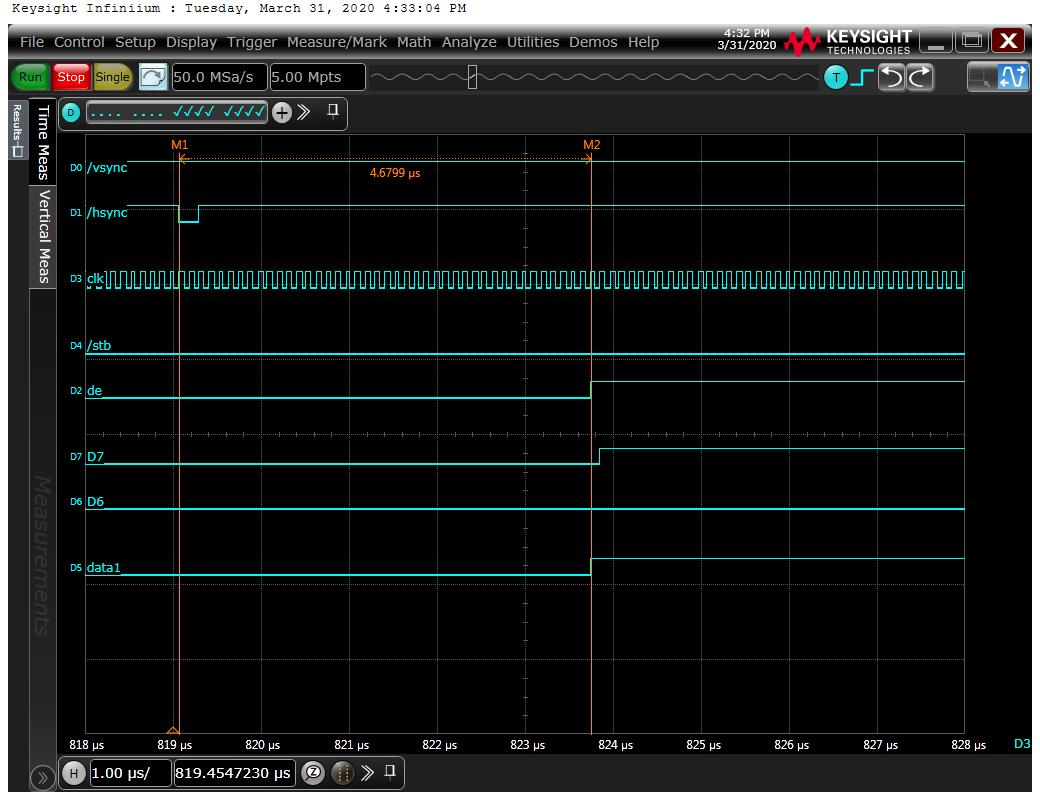
\includegraphics[width=14cm]{pictures/lcd_timings/hsync_falling_de_rising.jpg}
\end{center}
\caption{Time between ht-Sync falling edge and DE rising edge}
\label{fig:hsync_de}
\end{figure}
